\documentclass[tikz,border=8pt]{standalone}
% Shared look for every TikZ diagram. Load with % Shared look for every TikZ diagram. Load with % Shared look for every TikZ diagram. Load with \input{../../tools/tikz-style.tex}
\usepackage[T1]{fontenc}
\usepackage{lmodern}
\renewcommand{\sfdefault}{lmr}  % diagrams use the same serif as the text
\usetikzlibrary{arrows.meta, positioning, shapes.geometric, calc, fit, backgrounds}
\definecolor{cblue}{HTML}{4C78A8}
\definecolor{corange}{HTML}{F58518}
\definecolor{cgreen}{HTML}{54A24B}
\definecolor{cred}{HTML}{E45756}
\definecolor{cpurple}{HTML}{B279A2}
\definecolor{cgrey}{HTML}{6B6B6B}
\tikzset{
  every picture/.style={font=\sffamily, line width=1.2pt},
  box/.style={draw=#1, fill=#1!12, rounded corners=4pt, align=center, inner sep=7pt, minimum height=1.1cm},
  box/.default=cgrey,
  arrow/.style={-{Stealth[length=3mm]}, draw=cgrey, line width=1.4pt},
  title/.style={font=\sffamily\bfseries\Large},
  note/.style={font=\sffamily\small, text=cgrey, align=center},
}
\AtBeginDocument{\hyphenpenalty=10000 \exhyphenpenalty=10000}

\usepackage[T1]{fontenc}
\usepackage{lmodern}
\renewcommand{\sfdefault}{lmr}  % diagrams use the same serif as the text
\usetikzlibrary{arrows.meta, positioning, shapes.geometric, calc, fit, backgrounds}
\definecolor{cblue}{HTML}{4C78A8}
\definecolor{corange}{HTML}{F58518}
\definecolor{cgreen}{HTML}{54A24B}
\definecolor{cred}{HTML}{E45756}
\definecolor{cpurple}{HTML}{B279A2}
\definecolor{cgrey}{HTML}{6B6B6B}
\tikzset{
  every picture/.style={font=\sffamily, line width=1.2pt},
  box/.style={draw=#1, fill=#1!12, rounded corners=4pt, align=center, inner sep=7pt, minimum height=1.1cm},
  box/.default=cgrey,
  arrow/.style={-{Stealth[length=3mm]}, draw=cgrey, line width=1.4pt},
  title/.style={font=\sffamily\bfseries\Large},
  note/.style={font=\sffamily\small, text=cgrey, align=center},
}
\AtBeginDocument{\hyphenpenalty=10000 \exhyphenpenalty=10000}

\usepackage[T1]{fontenc}
\usepackage{lmodern}
\renewcommand{\sfdefault}{lmr}  % diagrams use the same serif as the text
\usetikzlibrary{arrows.meta, positioning, shapes.geometric, calc, fit, backgrounds}
\definecolor{cblue}{HTML}{4C78A8}
\definecolor{corange}{HTML}{F58518}
\definecolor{cgreen}{HTML}{54A24B}
\definecolor{cred}{HTML}{E45756}
\definecolor{cpurple}{HTML}{B279A2}
\definecolor{cgrey}{HTML}{6B6B6B}
\tikzset{
  every picture/.style={font=\sffamily, line width=1.2pt},
  box/.style={draw=#1, fill=#1!12, rounded corners=4pt, align=center, inner sep=7pt, minimum height=1.1cm},
  box/.default=cgrey,
  arrow/.style={-{Stealth[length=3mm]}, draw=cgrey, line width=1.4pt},
  title/.style={font=\sffamily\bfseries\Large},
  note/.style={font=\sffamily\small, text=cgrey, align=center},
}
\AtBeginDocument{\hyphenpenalty=10000 \exhyphenpenalty=10000}

% one column of cells: \col{x}{name}{colour}{v1,v2,...}
\newcommand{\col}[4]{
  \node[font=\sffamily\bfseries\small, text=#3] at (#1,0.6) {#2};
  \foreach \v [count=\i] in {#4} {
    \node[draw=#3, fill=#3!10, minimum width=3.4cm, minimum height=0.75cm] at (#1,-0.75*\i+0.35) {\v};
  }
}
\begin{document}
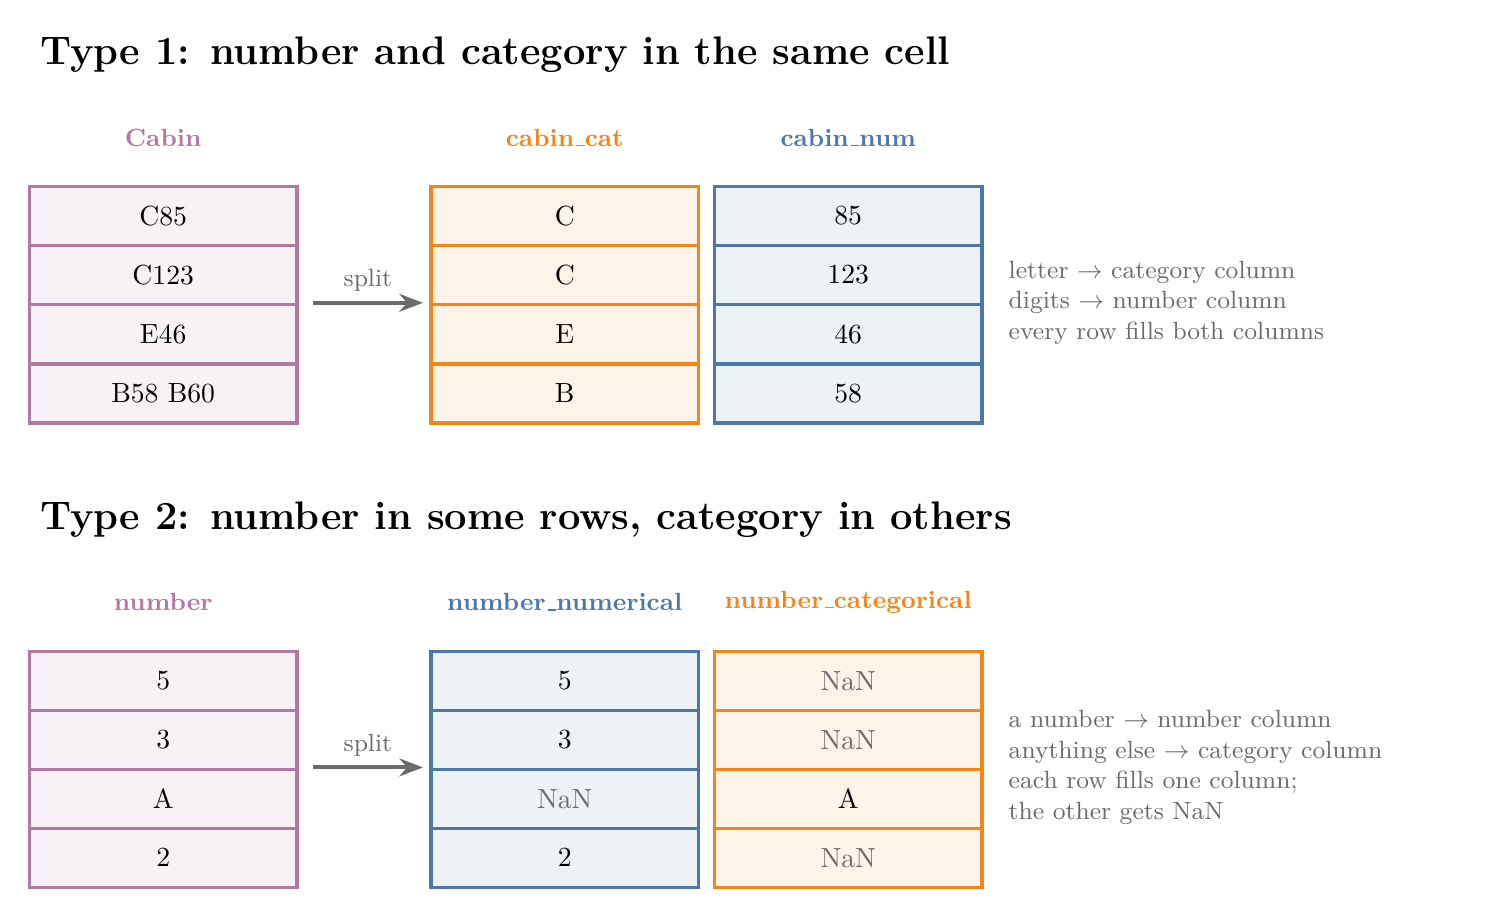
\begin{tikzpicture}
  % Type 1
  \node[title, anchor=west] at (-1.7,1.65) {Type 1: number and category in the same cell};
  \col{0}{Cabin}{cpurple}{C85, C123, E46, B58 B60}
  \draw[arrow] (1.9,-1.5) -- node[above, note] {split} (3.3,-1.5);
  \col{5.1}{cabin\_cat}{corange}{C, C, E, B}
  \col{8.7}{cabin\_num}{cblue}{85, 123, 46, 58}
  \node[note, anchor=west, text width=5.6cm, align=left] at (10.6,-1.5) {letter $\rightarrow$ category column\\ digits $\rightarrow$ number column\\ every row fills both columns};
  % Type 2
  \begin{scope}[yshift=-5.9cm]
  \node[title, anchor=west] at (-1.7,1.65) {Type 2: number in some rows, category in others};
  \col{0}{number}{cpurple}{5, 3, A, 2}
  \draw[arrow] (1.9,-1.5) -- node[above, note] {split} (3.3,-1.5);
  \col{5.1}{number\_numerical}{cblue}{5, 3, \textcolor{cgrey}{NaN}, 2}
  \col{8.7}{number\_categorical}{corange}{\textcolor{cgrey}{NaN}, \textcolor{cgrey}{NaN}, A, \textcolor{cgrey}{NaN}}
  \node[note, anchor=west, text width=5.6cm, align=left] at (10.6,-1.5) {a number $\rightarrow$ number column\\ anything else $\rightarrow$ category column\\ each row fills one column;\\ the other gets NaN};
  \end{scope}
\end{tikzpicture}
\end{document}
